% Compile with XeLaTeX:
%   latexmk -xelatex main.tex
% The project .latexmkrc automatically removes intermediate files afterwards
% (for example, main.aux, main.lof, and main.log), while keeping main.pdf.
\documentclass[11pt,a4paper]{article}

% -----------------------------------------------------------------------------
% Project information: update these fields before submission.
% -----------------------------------------------------------------------------
\newcommand{\CourseCode}{ME5411}
\newcommand{\CourseTitle}{Robot Vision and AI}
\newcommand{\ProjectTitle}{Group Project Report}
\newcommand{\AcademicYear}{Academic Year 2026/2027}
\newcommand{\GroupNumber}{17}
\newcommand{\SubmissionDate}{20 November 2026}

% Add or remove rows as needed. Keep the final \\ on every member row.
\newcommand{\GroupMembers}{%
  LI JIHAN & A0350821M \\
  HU ZHENG & Student Number 2 \\
  XU DARUI & Student Number 3 \\
  ZHAN CHENG  & Student Number 3 \\
}

% -----------------------------------------------------------------------------
% Font, page, and paragraph formatting required by the project brief.
% -----------------------------------------------------------------------------
\usepackage{fontspec}
% Install the actual Arial family with scripts/install_report_fonts.sh.
\setmainfont{Arial}
\setsansfont{Arial}

\usepackage[a4paper,margin=25mm,headheight=15pt]{geometry}
\usepackage{setspace}
\singlespacing
\setlength{\parindent}{1.5em}
\setlength{\parskip}{0.35em}
% Keep natural paragraph spacing on pages containing differently sized figures.
\raggedbottom
\setlength{\emergencystretch}{2em}

% -----------------------------------------------------------------------------
% Mathematics, tables, figures, and algorithms.
% -----------------------------------------------------------------------------
\usepackage{amsmath,amssymb}
\usepackage{graphicx}
\usepackage{booktabs}
\usepackage{array}
\usepackage{tabularx}
\usepackage{float}
\usepackage{placeins}
\usepackage{caption}
\usepackage{subcaption}
\usepackage{xcolor}
\usepackage{tikz}
\usetikzlibrary{arrows.meta,positioning,shapes.geometric}
\usepackage{cite}
\usepackage{enumitem}
\usepackage{xurl}
\usepackage{tocloft}
% The contents list needs only the task and subsection levels.
\setcounter{tocdepth}{2}
\setlength{\cftbeforesecskip}{2pt}
\setlength{\cftbeforesubsecskip}{0pt}

% Allow figures and text to share pages while keeping floats within each task.
\setcounter{topnumber}{3}
\setcounter{bottomnumber}{2}
\setcounter{totalnumber}{5}
\renewcommand{\topfraction}{0.9}
\renewcommand{\bottomfraction}{0.8}
\renewcommand{\textfraction}{0.08}
\renewcommand{\floatpagefraction}{0.75}
\setlength{\textfloatsep}{12pt plus 2pt minus 2pt}
\setlength{\floatsep}{10pt plus 2pt minus 2pt}
\setlength{\intextsep}{10pt plus 2pt minus 2pt}

\graphicspath{{figures/}{task_1/outputs/}{task_2/outputs/}{task_3/outputs/}%
  {task_4/outputs/}{task_5/outputs/}{task_6/outputs/}{task_7/outputs/}}

\captionsetup{
  font=normalfont,
  labelfont=bf,
  justification=centering,
  singlelinecheck=true
}
\setlist{nosep}

% Keep figures and tables numbered by report section.
\numberwithin{figure}{section}
\numberwithin{table}{section}
\numberwithin{equation}{section}

% -----------------------------------------------------------------------------
% Headings, links, and page style.
% -----------------------------------------------------------------------------
\usepackage{titlesec}
\titleformat{\section}
  {\normalfont\bfseries\Large}{\thesection}{0.75em}{}
\titleformat{\subsection}
  {\normalfont\bfseries\large}{\thesubsection}{0.75em}{}
\titleformat{\subsubsection}
  {\normalfont\bfseries\normalsize}{\thesubsubsection}{0.75em}{}
\titlespacing*{\section}{0pt}{2.0ex plus 0.5ex minus 0.2ex}{1.0ex}
\titlespacing*{\subsection}{0pt}{1.5ex plus 0.4ex minus 0.2ex}{0.8ex}
\titlespacing*{\subsubsection}{0pt}{1.2ex plus 0.3ex minus 0.2ex}{0.6ex}

\usepackage{fancyhdr}
\pagestyle{fancy}
\fancyhf{}
\fancyhead[L]{\CourseCode\ \CourseTitle}
\fancyhead[R]{Group \GroupNumber}
\fancyfoot[C]{\thepage}
\renewcommand{\headrulewidth}{0.4pt}
\renewcommand{\footrulewidth}{0pt}

\usepackage[hidelinks]{hyperref}
\hypersetup{
  pdftitle={\CourseCode\ \ProjectTitle},
  pdfauthor={Group \GroupNumber},
  pdfsubject={\CourseTitle},
  bookmarksnumbered=true,
  bookmarksopen=true
}
\usepackage[nameinlink,noabbrev]{cleveref}

% Task-boundary FloatBarriers preserve figure ownership without forcing a page.
\newcommand{\includetask}[3]{%
  \IfFileExists{#3}{%
    \FloatBarrier
    \section{Task #1: #2}
    \label{sec:task-#1}
    \input{#3}%
  }{}%
}

\begin{document}
\hypersetup{pageanchor=false}

% -----------------------------------------------------------------------------
% Title page
% -----------------------------------------------------------------------------
\begin{titlepage}
  \thispagestyle{empty}
  \centering

  \vspace*{18mm}
  {\Large National University of Singapore\par}
  \vspace{5mm}
  {\Large Department of Mechanical Engineering\par}

  \vfill
  {\LARGE\bfseries \CourseCode\ \CourseTitle\par}
  \vspace{8mm}
  {\Huge\bfseries \ProjectTitle\par}
  \vspace{6mm}
  {\Large \AcademicYear\par}

  \vfill
  {\Large\bfseries Group \GroupNumber\par}
  \vspace{8mm}

  \renewcommand{\arraystretch}{1.35}
  \begin{tabular}{>{\raggedright\arraybackslash}p{65mm}
                  >{\raggedright\arraybackslash}p{52mm}}
    \toprule
    \textbf{Name} & \textbf{Student Number} \\
    \midrule
    \GroupMembers
    \bottomrule
  \end{tabular}

  \vfill
  {\large Submission date: \SubmissionDate\par}
\end{titlepage}

% -----------------------------------------------------------------------------
% Front matter
% -----------------------------------------------------------------------------
\hypersetup{pageanchor=true}
\pagenumbering{roman}
\setcounter{page}{1}
\tableofcontents
\clearpage
\listoffigures
\listoftables

% -----------------------------------------------------------------------------
% Main report
% -----------------------------------------------------------------------------
\clearpage
\pagenumbering{arabic}
\setcounter{page}{1}

\section{Introduction}
\label{sec:introduction}
Recognising characters printed on microchips supports component identification
and visual inspection, but reliable recognition depends on both the image
processing pipeline and the classifier.  The supplied $990\times367$ chip
photograph contains the target row \texttt{HD44780A00}, with bright strokes on
a dark, non-uniform surface.  Ring-like texture and speckle noise overlap the
character intensity range, while weak strokes and narrow gaps make global
thresholding and character separation difficult.  This project investigates
how to preserve the character structure through enhancement, smoothing,
segmentation, and supervised recognition, and how decisions at each stage
affect the final result.

Tasks~1--6 develop the image-processing pipeline and compare alternative
methods using intermediate images and quantitative measurements.  Percentile
stretching, gamma correction, and histogram equalisation are evaluated before
averaging filters of several sizes are tested.  The selected 2--98\%
percentile stretch and $5\times5$ smoothing support projection-based
extraction of the character row.  Global Otsu and local adaptive thresholding
are then compared: the adaptive method preserves ten separate character
regions, whereas global thresholding merges neighbouring glyphs.
Moore-neighbour contour following extracts the character outlines, and
two-pass connected-component labelling with area filtering produces ten
labelled crops in reading order.  These experiments connect the quality of
the earlier preprocessing stages to the later segmentation outcome.

Task~7 compares a convolutional neural network (CNN) with a fully connected
multilayer perceptron (MLP) trained as a supervised regression model.  The MLP
regresses seven-dimensional one-hot targets with mean-square error, and three
independently trained members are combined by averaging their output scores.
The 7,112 labelled images in \texttt{dataset\_2026}, covering the classes
\texttt{0}, \texttt{4}, \texttt{7}, \texttt{8}, \texttt{A}, \texttt{D}, and
\texttt{H}, are divided into 75\% training and 25\% test sets.  Exact duplicate
images remain within one partition, and model selection uses validation data
drawn only from the training pool.  Both networks use input standardisation
and batch normalisation; input resolution and learning rate are investigated.
Accuracy, macro-F1, confusion matrices, parameter counts, and measured
training and inference times provide the effectiveness and efficiency
comparison.  The chip photograph and its segmented characters are reserved
for inference after training.

The selected CNN and MLP ensemble achieve held-out test accuracies of 99.33\%
and 98.71\%, respectively.  Direct grayscale inference on the photographed row
identifies one of ten characters with the CNN and nine with the MLP.  A further
class-independent preprocessing experiment uses the segmented binary
foreground and centres it at the median foreground dimensions estimated only
from the tuning-training images.  With the same trained models, this improves
the target-row results to eight of ten and ten of ten characters, respectively.
This ten-character check illustrates sensitivity to image appearance; it is
separate from the larger held-out test and does not establish general target-domain
accuracy.  Tasks~1--6 describe the
processing stages, \cref{sec:task-7} presents the learning experiments, and
\cref{sec:reproduction-guide} explains the implementation and reproduction
procedure.

\subsection{Processing and experimental workflows}
The two workflows show the image-processing dependencies and the separation
between training, model selection, evaluation, and inference.
\cref{fig:processing-workflow} follows the selected image-processing methods;
the Task~5 contour branch and Task~6 segmentation branch share the same binary
input.  \cref{fig:learning-workflow} shows that Figure~1 has no path into
training or model selection.

\begin{figure}[!htbp]
  \centering
  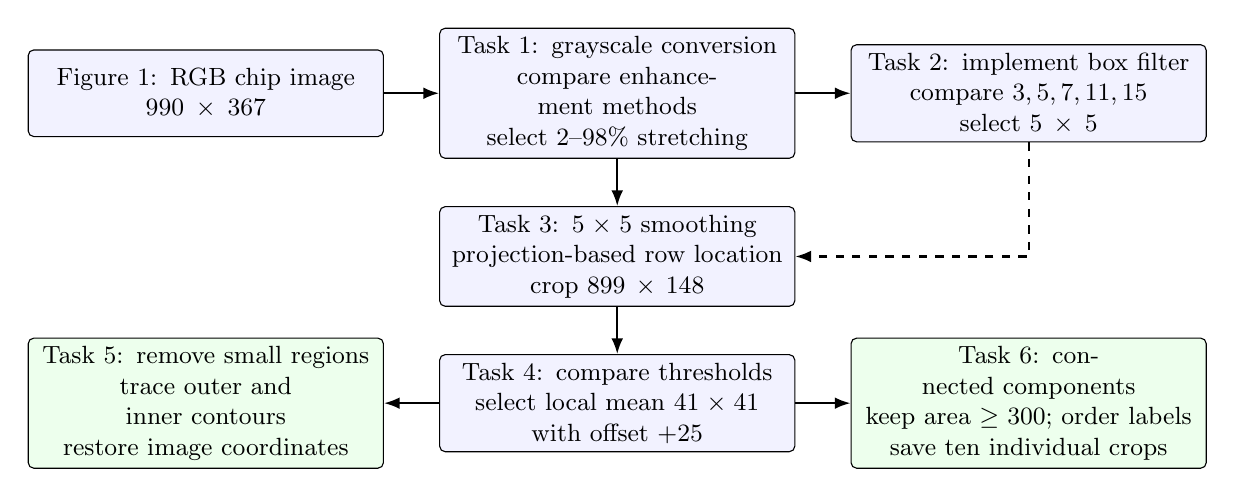
\begin{tikzpicture}[
    node distance=6mm and 7mm,
    block/.style={draw,rounded corners=2pt,fill=blue!5,align=center,
      text width=43mm,minimum height=11mm,font=\small,inner sep=3pt},
    output/.style={block,fill=green!7},
    arrow/.style={-{Latex[length=2mm]},thick}]
    \node[block] (input) {Figure~1: RGB chip image\\$990\times367$};
    \node[block,right=of input] (enhance) {Task~1: grayscale conversion\\compare enhancement methods\\select 2--98\% stretching};
    \node[block,right=of enhance] (smooth) {Task~2: implement box filter\\compare $3,5,7,11,15$\\select $5\times5$};
    \node[block,below=of enhance] (crop) {Task~3: $5\times5$ smoothing\\projection-based row location\\crop $899\times148$};
    \node[block,below=of crop] (binary) {Task~4: compare thresholds\\select local mean $41\times41$\\with offset $+25$};
    \node[output,left=of binary] (contour) {Task~5: remove small regions\\trace outer and inner contours\\restore image coordinates};
    \node[output,right=of binary] (segment) {Task~6: connected components\\keep area $\geq300$; order labels\\save ten individual crops};
    \draw[arrow] (input) -- (enhance);
    \draw[arrow] (enhance) -- (smooth);
    \draw[arrow] (enhance) -- (crop);
    \draw[arrow,dashed] (smooth.south) |- (crop.east);
    \draw[arrow] (crop) -- (binary);
    \draw[arrow] (binary) -- (contour);
    \draw[arrow] (binary) -- (segment);
  \end{tikzpicture}
  \caption{Selected Tasks~1--6 workflow. The dashed arrow transfers the
  selected filter setting; Task~3 applies that filter to Task~1's output.
  Task~5 and Task~6 are separate branches of the Task~4 binary image.}
  \label{fig:processing-workflow}
\end{figure}

\begin{figure}[!htbp]
  \centering
  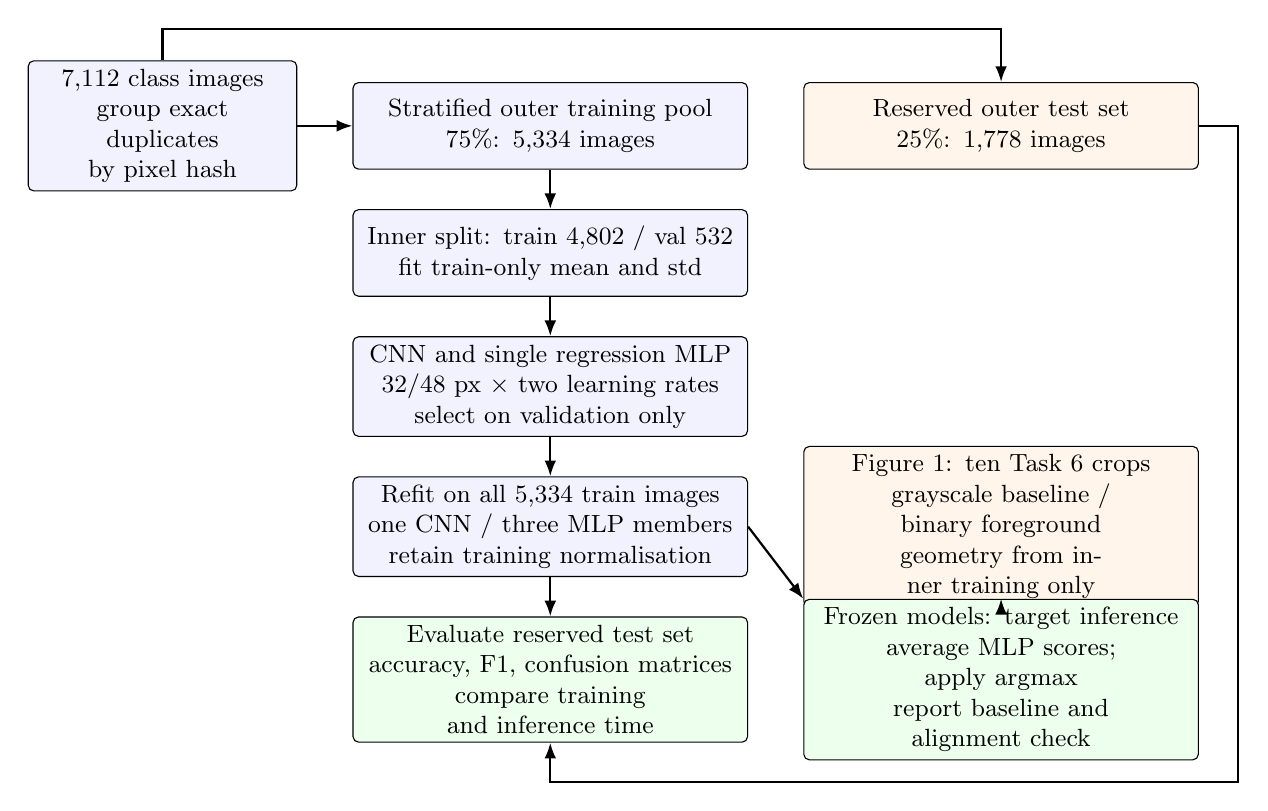
\begin{tikzpicture}[
    node distance=5mm and 7mm,
    block/.style={draw,rounded corners=2pt,fill=blue!5,align=center,
      text width=48mm,minimum height=11mm,font=\small,inner sep=3pt},
    held/.style={block,fill=orange!8},
    result/.style={block,fill=green!7},
    arrow/.style={-{Latex[length=2mm]},thick}]
    \node[block] (train) {Stratified outer training pool\\75\%: 5,334 images};
    \node[block,left=of train,text width=32mm] (data) {7,112 class images\\group exact duplicates\\by pixel hash};
    \node[held,right=of train] (test) {Reserved outer test set\\25\%: 1,778 images};
    \node[block,below=of train] (inner) {Inner split: train 4,802 / val 532\\fit train-only mean and std};
    \node[block,below=of inner] (tune) {CNN and single regression MLP\\$32/48$ px $\times$ two learning rates\\select on validation only};
    \node[block,below=of tune] (refit) {Refit on all 5,334 train images\\one CNN / three MLP members\\retain training normalisation};
    \node[result,below=of refit] (eval) {Evaluate reserved test set\\accuracy, F1, confusion matrices\\compare training and inference time};
    \node[held,right=of refit] (target) {Figure~1: ten Task~6 crops\\grayscale baseline / binary foreground\\geometry from inner training only};
    \node[result,right=of eval] (infer) {Frozen models: target inference\\average MLP scores; apply argmax\\report baseline and alignment check};
    \draw[arrow] (data) -- (train);
    \draw[arrow] (data.north) -- ++(0,4mm) -| (test.north);
    \draw[arrow] (train) -- (inner);
    \draw[arrow] (inner) -- (tune);
    \draw[arrow] (tune) -- (refit);
    \draw[arrow] (refit) -- (eval);
    \draw[arrow] (test.east) -- ++(5mm,0)
      |- ([yshift=-5mm]eval.south) -- (eval.south);
    \draw[arrow] (target) -- (infer);
    \draw[arrow] (refit.east) -- (infer.north west);
  \end{tikzpicture}
  \caption{Task~7 experimental workflow. The outer test set and Figure~1
  are excluded from optimisation and model selection. Target geometry
  alignment uses only statistics of the inner training images.}
  \label{fig:learning-workflow}
\end{figure}
\FloatBarrier


\includetask{1}{Original Image and Contrast Enhancement}{task_1/task_1.tex}
\includetask{2}{Image Smoothing with Averaging Filters}{task_2/task_2.tex}
\includetask{3}{Sub-image Extraction}{task_3/task_3.tex}
\includetask{4}{Binary Image Conversion}{task_4/task_4.tex}
\includetask{5}{Character Outline Detection}{task_5/task_5.tex}
\includetask{6}{Character Segmentation and Labelling}{task_6/task_6.tex}
\includetask{7}{Character Classification}{task_7/task_7.tex}

\section{Implementation and Reproduction Guide}
\label{sec:reproduction-guide}
The Python implementation is reproduced from the repository root (the
directory containing \path{main.tex} and \path{common.py}) as follows.
Each task has an entry-point script, a report fragment, implementation notes,
and an \path{outputs/} directory.

\begin{enumerate}[leftmargin=*,itemsep=0.5em]
\item \textbf{Check the supplied data.}
Place \path{Test_Image_2026.bmp} in \path{dataset_2026/}, alongside the seven
class directories \texttt{0, 4, 7, 8, A, D, H}.  Each class contains 1,016
PNG images (7,112 images in total), with source dimensions $128\times128$.
Keep the BMP and its derived crops outside the labelled directories: they are
reserved for Figure~1 inference.

\item \textbf{Create the software environment.}
Install Conda, then execute:
{\small
\begin{verbatim}
conda env create -f task_7/environment.yml
source "$(conda info --base)/etc/profile.d/conda.sh"
conda activate cvtask
\end{verbatim}
}
If \texttt{cvtask} already exists, replace the creation command with
\texttt{conda env update -n cvtask -f task\_7/environment.yml}.
The environment file pins Python~3.8, PyTorch~2.0.0, torchvision~0.15.1~\cite{torchvision},
CUDA runtime~11.8, NumPy~1.24.2, Pillow~9.4.0, and Matplotlib~3.7.1.
The measured runtime was Ubuntu~20.04, Python~3.8.10, and
PyTorch~2.0.0+cu118 on an NVIDIA GeForce RTX~4080 SUPER.
Tasks~1--6 run on the CPU.  Task~7 automatically selects CUDA if available,
otherwise the CPU; prefixing its command with
\texttt{CUDA\_VISIBLE\_DEVICES=""} forces CPU execution.  Timings are
device-dependent.  Plots use the Agg backend and require no display server.

\item \textbf{Run every image-processing stage in order.}
{\small
\begin{verbatim}
python task_1/task_1.py
python task_2/task_2.py
python task_3/task_3.py
python task_4/task_4.py
python task_5/task_5.py
python task_6/task_6.py
\end{verbatim}
}
These scripts create or replace files in their fixed
\path{task_N/outputs/} directories.  Task~1 reads the BMP and saves
\path{task1_percentile_stretch_p02_p98.png} for Tasks~2 and~3.
Task~2 is the filter-size comparison branch; Task~3 uses the Task~1 enhanced
image and original BMP to save \path{task_3/outputs/task3_subimage.png}.
Task~4 produces \path{task_4/outputs/task4_binary.png} and the Otsu comparison.
Tasks~5 and~6 read the Task~3 grayscale image and Task~4 binary results.
Task~5 writes outline figures and JSON contour records.
Task~6 writes \path{task6_components.csv} and ten pairs of
\path{task_6/outputs/chars/char_*_gray.png} and \path{char_*_bin.png} crops;
these must exist before Task~7 to obtain the Figure~1 recognition results.

\item \textbf{Run the complete learning experiment.}
Use a separate directory to preserve the report's supplied results:
{\small
\begin{verbatim}
python task_7/task_7.py --data dataset_2026 \
  --output task_7/outputs_reproduction
\end{verbatim}
}
The default seed is 20261013, batch size 128, tuning limit 18 epochs,
early-stopping patience 5, and data-loader workers 0.  The full run performs
the $32/48$-pixel and $10^{-3}/3\times10^{-4}$ learning-rate grid, chooses
models on validation data, refits on the full 75\% training pool using the
selected validation epoch, then evaluates the 25\% test partition and the
target crops.  It uses one CNN and three MLP regression members.
For a short pipeline check, use:
{\small
\begin{verbatim}
python task_7/task_7.py --data dataset_2026 \
  --smoke --output task_7/outputs_smoke
\end{verbatim}
}
Smoke mode uses one input size, one learning rate, at most two tuning epochs,
and one MLP; it is not the reported experiment.  Always specify the smoke
directory because the default output is \path{task_7/outputs/}.
The main artifacts are \path{split_summary.json} and
\path{split_manifest.csv} (partition audit), \path{tuning_results.csv} and
\path{tuning_curves.png} (model selection), \path{task7_metrics.json} and
\path{method_comparison.csv} (results and timing), two confusion-matrix PNGs,
\path{*.pt} checkpoints, and \path{target_predictions.json}.
The report reads its formal figures from \path{task_7/outputs/}; independent
reproduction and smoke runs leave these unchanged.  Replacing the formal
directory requires updating the report's numerical tables to match the new
metrics.  Exact numerical agreement and timing across different software or
hardware are not guaranteed.

To repeat target inference from the supplied models without retraining, copy
\path{task_7/outputs/} to a new \path{task_7/outputs_inference_check/}
directory, then run:
{\small
\begin{verbatim}
python task_7/task_7.py --data dataset_2026 --inference-only \
  --output task_7/outputs_inference_check
\end{verbatim}
}
This mode needs both crop variants, the dataset, split manifest, and copied
checkpoints.  It fits foreground geometry from training rows only and updates
target inference while preserving test metrics and the grayscale baseline.

\item \textbf{Compile the report.}
Install XeLaTeX, latexmk, and the recommended/extra LaTeX packages.
On Ubuntu, run:
{\small
\begin{verbatim}
sudo apt-get install latexmk texlive-xetex texlive-latex-extra \
  texlive-latex-recommended texlive-fonts-recommended \
  curl cabextract fontconfig
\end{verbatim}
}
Omit \texttt{sudo} when running as root.  The provided font installer verifies
and installs the actual Arial family (regular, bold, italic, and bold italic)
under \path{~/.local/share/fonts/msttcorefonts/} by default, without root
privileges; \texttt{REPORT\_FONT\_DIR} can override the directory.
With all task figures present, execute:
{\small
\begin{verbatim}
bash scripts/install_report_fonts.sh
fc-match Arial
latexmk -xelatex -interaction=nonstopmode -halt-on-error \
  -file-line-error main.tex
\end{verbatim}
}
The font check must resolve to Arial.  The build also runs BibTeX for the
references.  The output is \path{main.pdf}.  The project \path{.latexmkrc} removes auxiliary
build files after a successful build while retaining the PDF.
\end{enumerate}

\noindent\path{README.md} contains the full directory dependency table,
artifact inventory, version-check command, and build troubleshooting command.


\section{Discussion and Conclusion}
\label{sec:discussion}
Tasks~1--6 taught us how image-processing functions relate to measurable image
properties.  Grayscale conversion and contrast transforms change intensity
distributions; averaging reduces local variation but also weakens edge
gradients.  Row and column projections describe text location, while
thresholding determines foreground connectivity.  Contour following exposes
boundaries and holes, and connected-component labelling uses adjacency, area,
and bounding boxes to separate characters.  These relationships explain why
each stage must preserve the information needed by the next stage, rather
than merely produce a visually smoother or brighter image.

The comparisons support the selected pipeline.  In Task~1, percentile
stretching gave better character-to-background separation than histogram
equalisation, which amplified texture; gamma correction produced a smaller
improvement.  Task~2 showed the noise--detail trade-off: larger averaging
kernels suppressed more noise but blurred strokes, so $5\times5$ was a
practical compromise.  In Task~3, band-adaptive refinement reduced the effect
of texture on coarse projection-based localisation, and a safety margin
preserved the complete row.  In Task~4, smoothing and opening reduced Otsu
noise but left only seven merged character groups; local adaptive thresholding
retained ten.  Tasks~5 and~6 showed that correct component counts do not
guarantee intact glyph topology: the open lower loop of \texttt{8} and tiny
holes in \texttt{0} remained visible in the contours.  Area filtering removed
the much smaller noise regions, enabling ten separately labelled crops.

Our investigations also covered the mathematical definitions of the methods:
grayscale weighting, percentile and gamma transforms, cumulative-histogram
mapping, neighbourhood averaging, projection sums, threshold criteria,
morphological operations, contour traversal, and component equivalence.
The preceding task sections document these formulations and implementation
rules.  We examined how NumPy supports array operations and statistics,
Pillow handles image decoding and resizing, Matplotlib presents results,
and PyTorch supplies networks, losses, automatic differentiation, and
optimisation~\cite{numpy,pillow,matplotlib,pytorch}.  The network investigation
included standardisation, BatchNorm, Dropout, one-hot MSE regression,
cross-entropy, and the actual hidden-layer activations:
\[
  \operatorname{ReLU}(z)=\max(0,z),\qquad
  \operatorname{GELU}(z)=z\Phi(z)
  =\frac{z}{2}\left[1+\operatorname{erf}\!\left(\frac{z}{\sqrt{2}}\right)\right].
\]
Here $\Phi$ is the standard normal cumulative distribution function.
The CNN uses ReLU's hard zero cutoff; the MLP uses GELU's smooth
weighting~\cite{gelu}.  Both have linear output layers, with argmax used for
the final class decision.  These are investigated design choices; their
individual benefits were not isolated through activation or regularisation
ablation experiments.

Task~7's CNN achieved slightly higher held-out accuracy than the MLP ensemble
(99.33\% versus 98.71\%).  The ensemble took longer to train, while its
lower-resolution input gave faster measured inference in this experiment.
Resolution and learning-rate effects depended on the configuration, and
single-run results limit the strength of sensitivity claims.  On Figure~1,
training-derived foreground alignment improved CNN recognition from one to
eight correct characters and MLP recognition from nine to ten, using unchanged
models.  This illustrates the importance of matching foreground appearance
and scale to the training data.  The project therefore achieved a complete
processing and recognition pipeline, while also showing that high accuracy
on clean data does not ensure reliable recognition of textured photographs;
the ten-character target check requires broader validation before general
claims can be made.

\FloatBarrier
\phantomsection
\addcontentsline{toc}{section}{References}
\bibliographystyle{unsrt}
\bibliography{references}

\end{document}
